\chapter{Research question}

The aim of this bachelor thesis is to perform research into chatbots and investigate how they are built. What actually goes into building a chatbot that feels intuitive but is also functional?

\section{Approach}

This thesis will start with some use cases for chatbots, to find out when it would be a good idea to build a chatbot as a solution for a concrete problem.

Already existing chatbots will be presented and compared to paint a picture of what professional chatbots currently look like.
Some general research into chatbot best practices will also be conducted based on real life cases

Finally, different platforms and frameworks to create a fully-fledged chatbot will be compared by building food ordering chatbot.

\section{Metrics}

The metrics for the comparison will be based on a number of different factors. Their general business model will be researched, followed by their learning curve and quality of documentation. Finally source code readability and scalability will be compared.

\chapter{General chatbot design}

\section{Choosing a chatbot solution}

\subsection{Introduction}

Why choose a chatbot as a solution to a problem? To find the answer to that question there should be a concrete description of the problem and research should be conducted into how that problem is currently handled.

\subsection{Use case 1: Food delivery}

Food delivery chatbots are some of the most common chatbots out there. That's because a basic chatbot for ordering food is easy to make and maintain. Most of the time they don't require complex language recognition and they will go through the same steps every time someone wants to order something.

A great example of this is Domino's\cite{dominos}. They own one of the most popular facebook messenger chatbots even though the bot itself is really simple.

Let's take a look at the perspective of a new imaginary pizza place in town. This pizza place has a set menu with set formulas. They want to innovate and make it possible to receive and process online orders but don't want to lose the familiarity of their brand.

This is a perfect case for a chatbot. If they already have a facebook page, they can easily integrate a chatbot into it and promote it to their current customers. All they need on top of that is an admin panel for the company to maintain their menu and process orders.

Building a chatbot this way also opens up several possibilities for expansion in the future. They can easily start tracking customer's habits and improve their suggestions for specific customers.

However there are some downsides to this solution as well. Creating a chatbot from scratch for this purpose would cost a lot of money. That's why there are already solutions like Chatobook~\cite{chatobook} popping up. This is an all-in-one solution that provides a restaurant with a messenger bot and an admin panel to manage promotion, reservations and the menu. You can also find templates for these kinds of bots that integrate with Google Sheets/Excel.~\cite{chatbot-templates-pizza}

The rise of general delivery services like Ubereats~\cite{ubereats} and Deliveroo~\cite{deliveroo} also complicates this matter. If those companies manage to integrate full ordering services into their platforms using chatbots -which they will most likely succeed in at one point- that would simplify everything. But that also comes with a cost. The imaginary pizza restaurant would lose its unique identity as the chatbot's identity would be replaced with Uber's or Deliveroo's identity.

\subsection{Use case 2: Banking industry}

Next case relates to the banking industry. Lately there has been an influx of integrating AI-powered chatbots into this sector. This is because people like to engage with their bank and get answers that feel human, instantly. It establishes a kind of trust. This type of communication is also very attractive to the banks themselves, because it allows them to quickly provide answers to repetitive questions.

There are lots of specific chatbot banking use cases out there. One of them is basic banking services. Checking account balance, transferring funds, analyzing expenditures. Chatbots can also hugely improve a bank's customer support, which should be available 24/7. They can help out people instantly, without long wait times which a lot of customer support services are currently struggling with. Further more, there's also the opportunity for intranet-based chatbots~\cite{intranet-chabot}. These chatbots communicate with the employees to improve their productivity and give them access to the right information in mere seconds. As seen in figure~\ref{fig:chatbot-benefit-graph2} customer service within a company is one of the business functions that can benefit the most from a chatbot.

Another use case is providing customer-focused marketing. Using a chatbot, it's possible to promote personalized banking services as if the customer is talking to a real life employee.

Overall, integrating a chatbot into a banking environment has a lot of benefits. That's why more and more banks are starting to invest in them.

\subsection{Use case 3: E-commerce}

Lastly there's the quickly growing industry of E-commerce. This ties into both of the use cases above as the main focus is customer interaction and engagement, support and personalized marketing.

Online web-stores are one of the fastest growing industries, they are popping up everywhere. This is because more and more people are starting to buy online. It's convenient, fast and reliable (in most cases). However there is one key benefit missing compared to in-store shopping: interaction.

Here's where the shopping assistant chatbot comes in. It can do everything a normal store employee can and even more. Like instantly retrieving your past orders to help you out quicker and more efficiently. It has access to every single product the web-shop offers and can instantly recommend one or more products that fit your needs. It can seamlessly provide post-purchase customer support. All of this whilst not losing the brand identity of the web-store itself.

As seen in the first figure~\ref{fig:chatbot-benefit-graph}, E-commerce is projected to be the industry that will benefit the most from chatbots. Anything involving the sale of goods or services online can be considered E-commerce. If a business corresponds to that description, experimenting with a chatbot could be interesting.

\subsection{Conclusion}

Chatbots are an obvious answer to lots of companies that are willing to innovate and are ready to experiment. It allows them to establish their brand in a familiar and human way, whilst also increasing their in-company productivity and overall efficiency.

\begin{figure}[p]
	\centering
	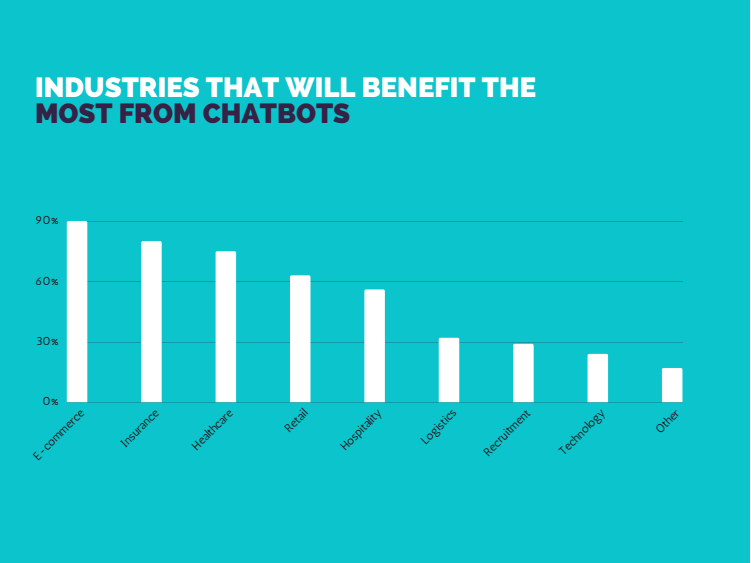
\includegraphics[width=\textwidth]{chatbot-benefit-graph2}\label{fig:chatbot-benefit-graph2}
	\caption{Industries projected to benefit from chatbots~\cite{chatbot-industry-benefits}}
\end{figure}

\begin{figure}[p]
	\centering
	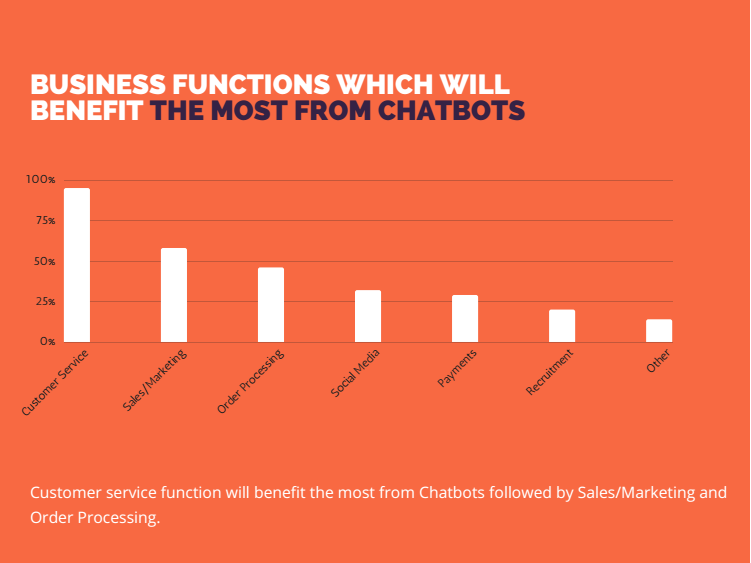
\includegraphics[width=\textwidth]{chatbot-benefit-graph}\label{fig:chatbot-benefit-graph}
	\caption{Business functions inside a company projected to benefit from chatbots~\cite{chatbot-industry-benefits}}
\end{figure}

\newpage

\section{Comparison of existing chatbots}

Today there are plenty of well-implemented solutions already. There's food-ordering services like Domino's that offer an ordering service. But also stores, ranging from specific ones (H\&M) to big, fully fledged web-stores like Bol.com, a Dutch-Belgian web-store.

\subsection{Dom, Domino's ordering assistant bot}

This is a facebook messenger bot for ordering food from Domino's, a fast food chain. Something that can immediately be noticed is the use of tappable quick reply answers. The bot starts with some simple questions in order to know the user's intent and asks some information about the user, such as the address and what store he or she wants to order from.

Once this has been established, the user can choose what he wants to order and checkout.

In conclusion, the bot isn't very smart. It simply takes orders and passes them through to the store. The user needs to follow the steps clearly and in the right order. It doesn't mimic a real life conversation. Some improvements would be building a profile of the user using past orders and providing recommendations. It could also keep you updated on new items being released. This would make the user feel more at home and establish a sort of familiarity with the bot, like he would with a normal employee.

\subsection{Bol.com, Customer support bot}

This bot's main focus lies in customer service. It replaces the long list of frequently asked questions that most customers really don't want to go through to find their answer. The bot also keeps your past and current orders in mind and integrates them into the conversation.

The bot keeps a very friendly and familiar tone towards the user throughout the entire conversation.

The language recognition seems to be focused on single word recognition to link the question to an answer. It also keeps spelling errors into account.

\section{Best practices}

\subsection{Creating a personality}

One of the most important factors in creating a chatbot is to develop a personality for it. This makes the bot a lot more engaging to the users and makes it harder for the user to get frustrated.

If there is already a company personality in place, the chatbot should get its traits there. If that's not the case, adding a name or a face, which doesn't necessarily have to be human, to it can already be a huge help.

\subsection{Making the conversation flow}

Conversations with a chatbot aren't as straight forward as they seem to be. Users can easily get distracted, overwhelmed or annoyed by a chatbot.

It is clear that a lot of research and testing should be performed into the conversational flow. A bad example of this is not having any wait time between messages. This overwhelms the user as he doesn't have time to read the previous message. Adding typing bubbles between messages not only gives the user time to read the previous message, but it also humanizes the bot.

\subsection{Predicting failure and user behavior}

Predicting failure and user behavior is hard in any user interface. But there are some common mistakes in chatbots that can be avoided even before testing.

There are several ways to handle unexpected user input.
One of them is revisiting the previous state of the conversation, another one is restarting the conversation, or asking the user politely what he's trying to accomplish.

Conversations that end up in this path should also be logged for evaluation afterwards to avoid future dead ends.

When using buttons in a bot, for example to visit a website, or start the conversation, they should be functional at all times.

Facebook's messenger platform supports 2 main buttons in their platform. General buttons, and quick replies. Regular buttons will always be clickable multiple times. Quick replies are bound to the message they are meant to follow up on, and disappear as soon as they are clicked.

Of course this best practice goes hand in hand with actual user testing and applies to every user interface, not just to chatbots.